% Teilauswertung 1

\section{Justage Dunkelfeldmikroskop}
Zu Beginn des Versuches musste das Dunkelfeldmikroskop justiert werden. Begonnen wurde mit der Justage der ersten Linse, hierfür wurde ein Beamsplitter mit Kamera vor der ersten Linse eingesetzt. Die Linse wurde so eingestellt, dass das Bild der Kamera möglichst scharf ist. Danach wurde die zweite Linse auf ähnliche weise eingestellt. Die Kamera befand sich zu diesem Zeitpunkt wieder auf der Ausgangsposition. Abschließend wurden noch zwei Spiegel benutzt, um den Lichtstrahl in das Spektrometer zu leiten.

%\newpage
\section{Vergleich Hell-/Dunkelfeldaufnahmen}
Im folgendem soll ein Vergleich zwischen Hell- bzw. Dunkelfeldmodus gezogen werden.

Abbildung \ref{fig:312-HF} zeigt eine Hellfeldaufnahme der Probe, der Marker ist als dunkles Kreuz zu erkennen, während der Hintergrund hell ist. Daneben sind die Verunreinigungen als schwarze Flecken zu erkennen. Die Felder der Probe sind dagegen nur schwer zu erkennen.
\begin{figure}[h]
    \centering
    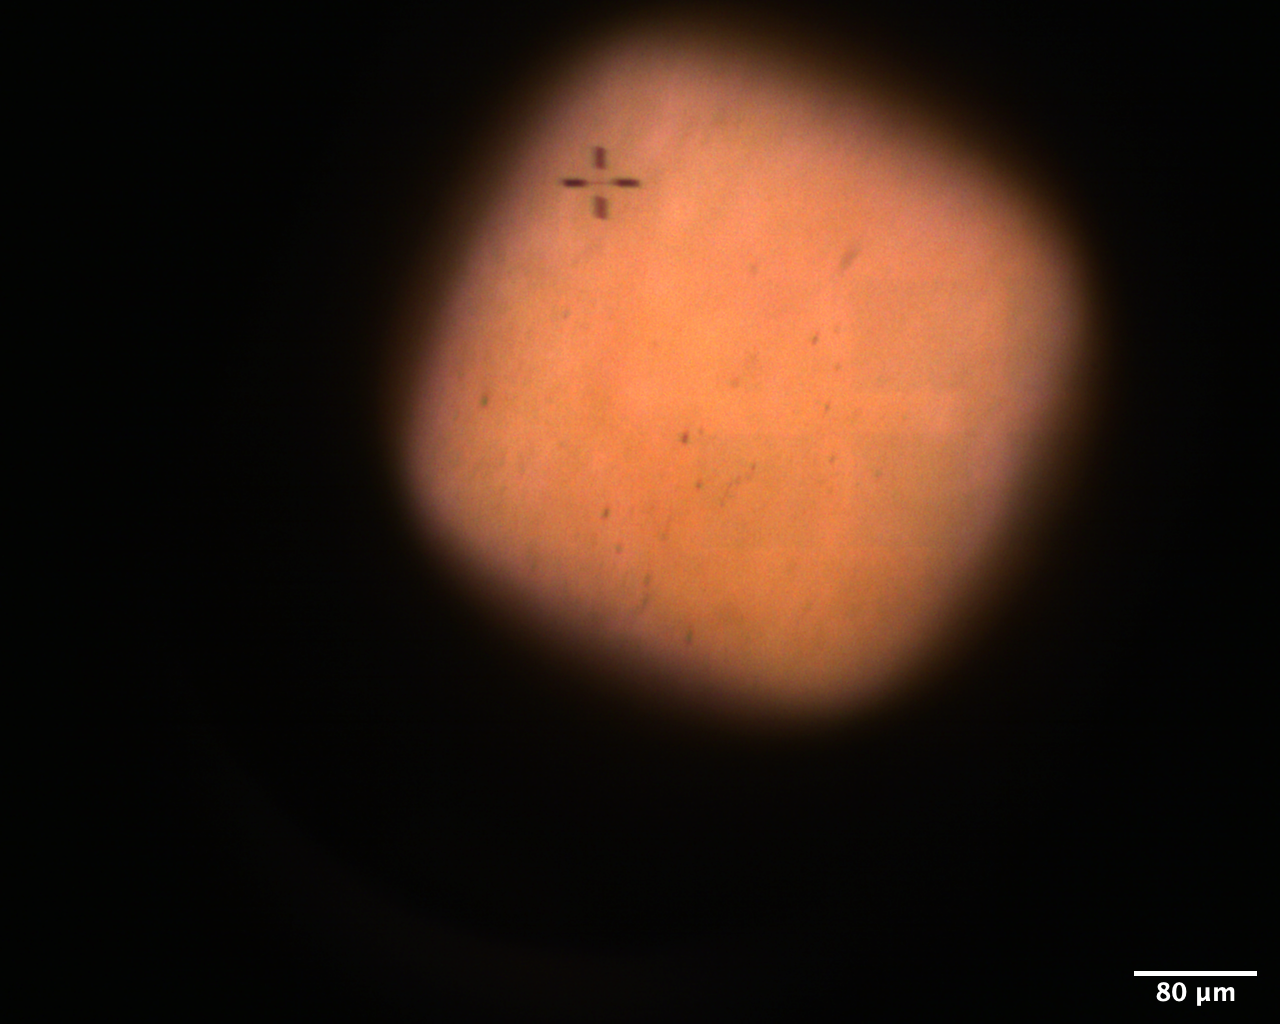
\includegraphics[width=0.5\textwidth]{Bilder/Auswertung/3.1/image_0.png}
    \caption{Hellfeldaufnahme einer Probe. Der Marker ist als Schatten zu sehen, die Felder sind als rechteckige Schatten kaum zu erkennen. Außerdem fallen weitere Dunkle stellen auf welche wahrscheinlich durch Verunreinigungen verursacht wurden.}
    \label{fig:312-HF}
\end{figure}

\newpage
Anders verhält sich dies in Abbildung \ref{fig:312-DF}, hier handelt es sich un eine Dunkelfelaufnahme der gleichen Probe. Wie zu erwarten war ist der Hintergrund nun dunkel, wohingegen die auf der Probe aufgebrachten Substanzen durch Streuung als Hell hervortreten. Der Marker ist hierbei am deutlichsten zu erkennen, gefolgt von hellen Flecken, die wahrscheinlich durch Verunreinigungen auf der Probe verursacht werden. Die Felder der Probe treten auch hier nicht sonderlich hervor, sind aber jedoch besser zu erkennen als im Hellfeldmodus.
\begin{figure}[h]

    \centering
    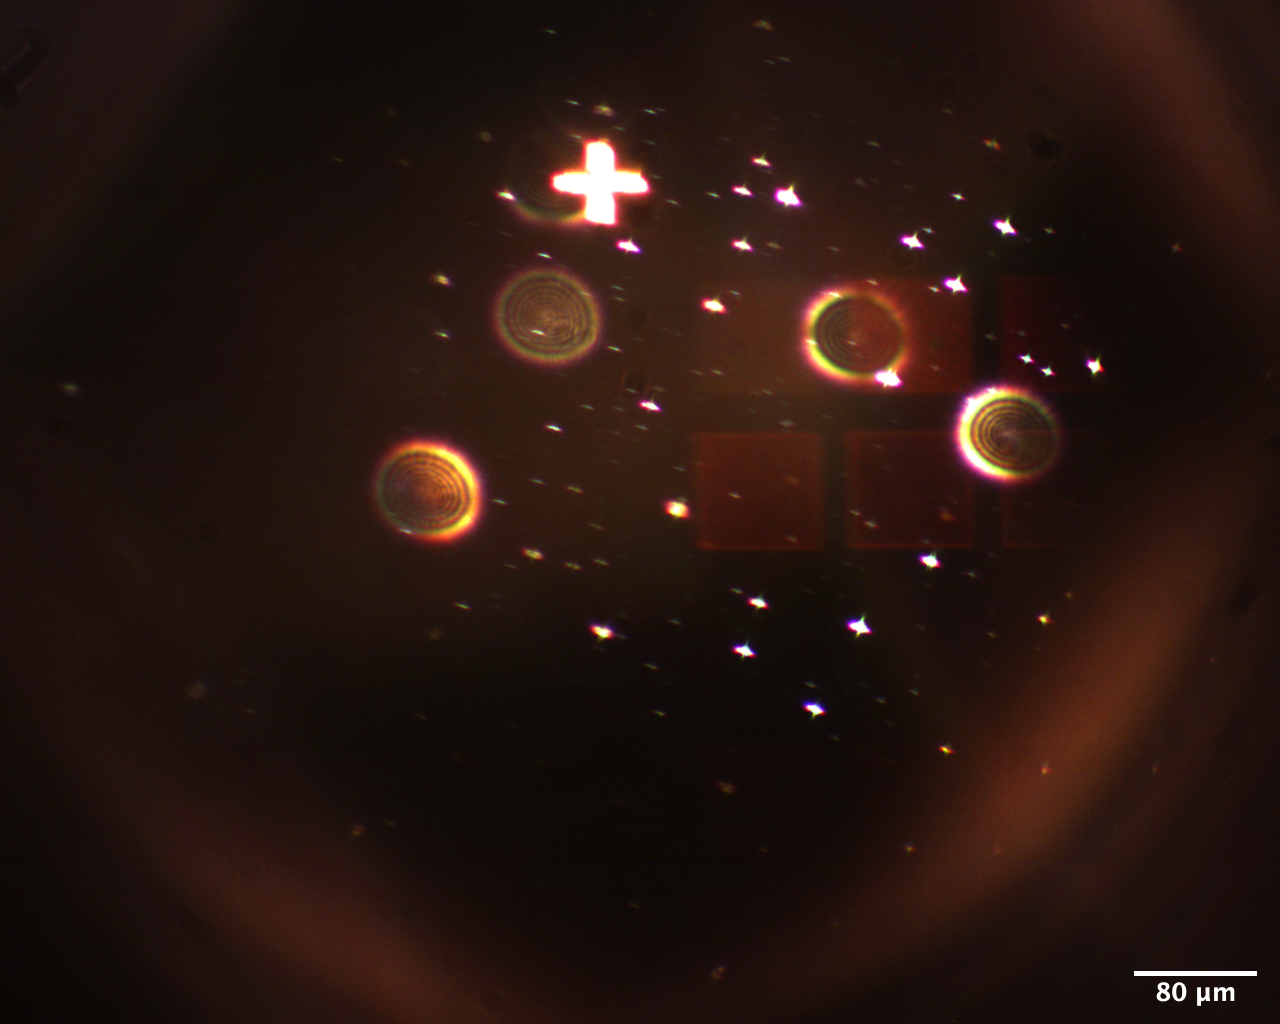
\includegraphics[width=0.5\textwidth]{Bilder/Auswertung/3.1/image_1.png}
    \caption{Dunkelfeldaufnahme einer Probe. Der Marker hebt sich durch eine hohe Helligkeit vom dunklen Hintergrund ab. Die Felder sind als hellere Quadrate zu erkennen. Daneben fallen weitere helle Flecken auf, welche wahrscheinlich auf Verunreinigungen zurückzuführen sind.}
    \label{fig:312-DF}
\end{figure}

\newpage
\section{Einfluss der Polarisation}
Beim Betrachten der Aufnahmen der Proben unter Verwendung von polarisierten Licht fällt auf, dass die Streuung für eine Polarisation von 0 Grad geringer ist als für 90 Grad. Im Allgemeinen sind die Proben mit eingesetztem Polfilter etwas dunkler.
\begin{figure}[h]
    \centering
    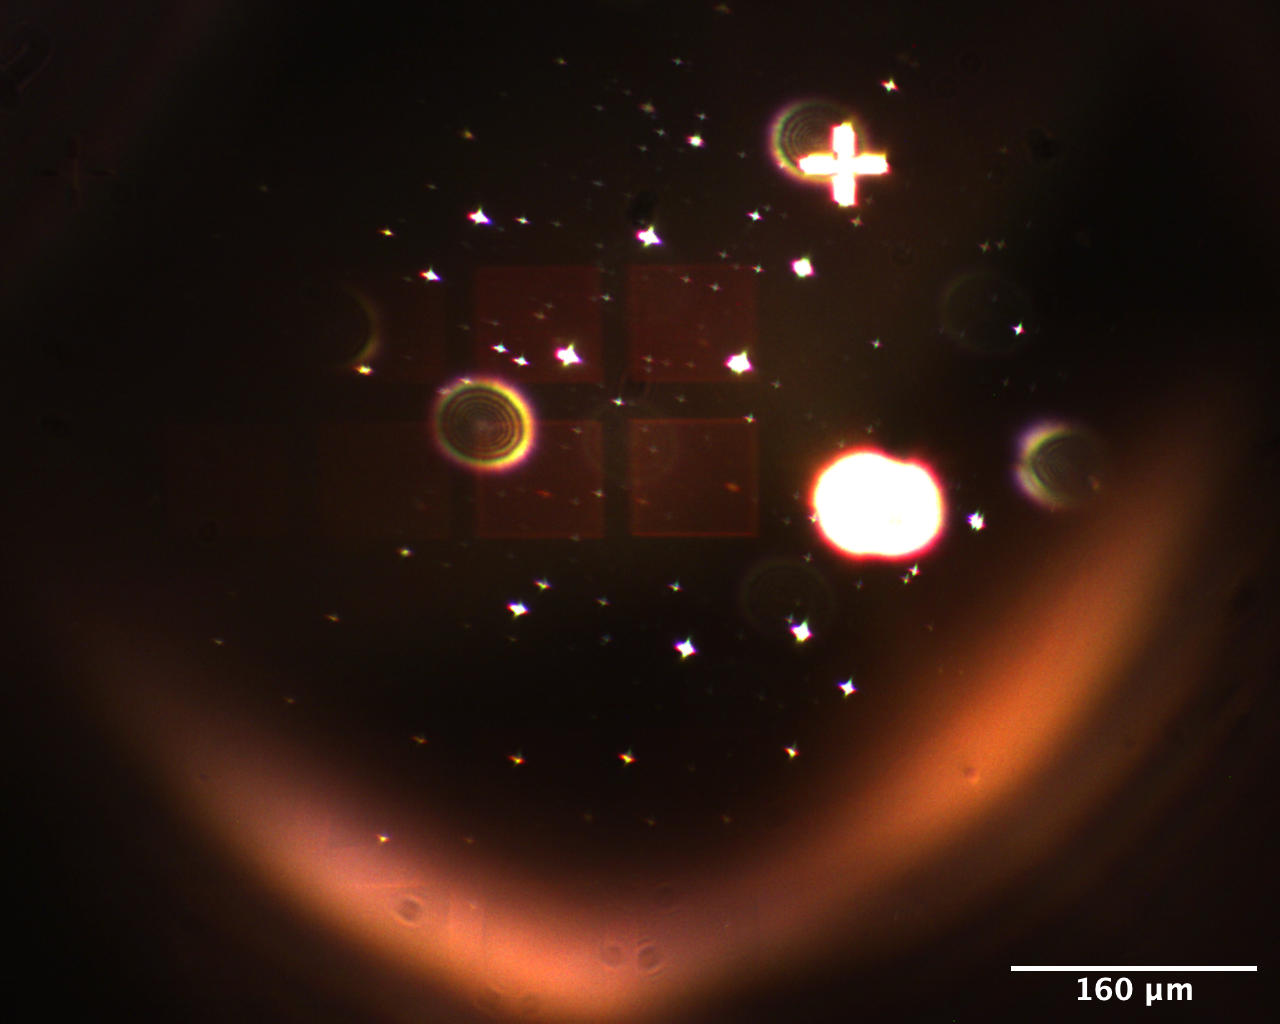
\includegraphics[width=0.5\textwidth]{Bilder/Auswertung/3.1/POL-0-image_2.png}
    \caption{Dunkelfeldaufnahme bei 0 Grad Polarisation.}
    \label{fig:314-POL0}
\end{figure}

\begin{figure}[h]
    \centering
    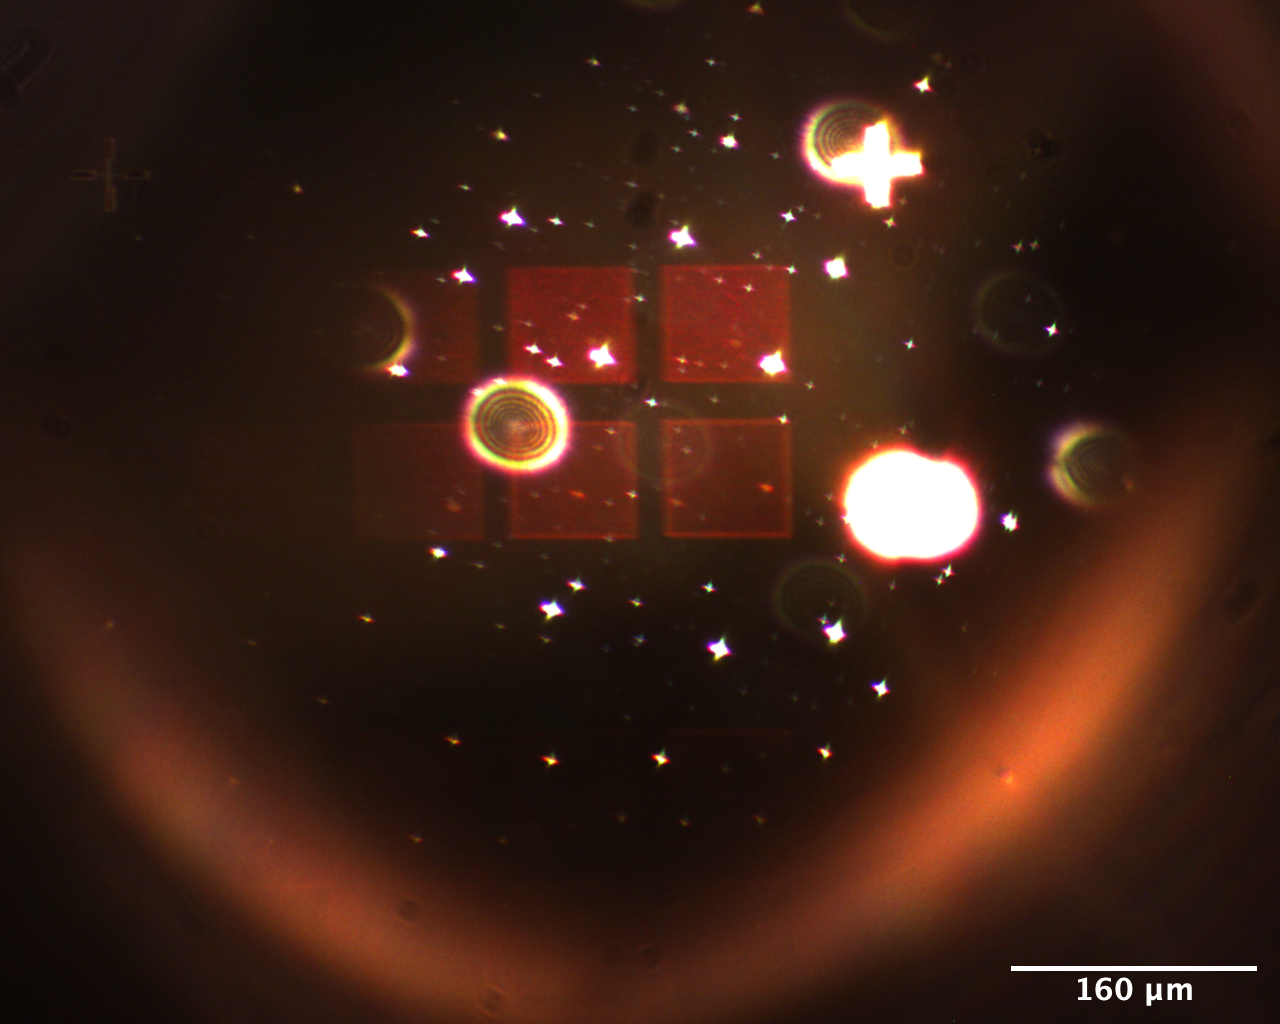
\includegraphics[width=0.5\textwidth]{Bilder/Auswertung/3.1/POL-90-image_3.png}
    \caption{Dunkelfeldaufnahme bei 90 Grad Polarisation.}
    \label{fig:314-POL90}
\end{figure}